\documentclass[a4paper, 11pt, twoside, table]{article}


% Police standard sous LaTeX : Latin Modern
\usepackage{lmodern} 
% (alternative à la police d'origine développée par Donald Knuth : Computer Modern)
\usepackage[french]{babel} % Pour la langue française
\usepackage[utf8]{inputenc} % Pour l'UTF-8
\usepackage[T1]{fontenc} % Pour les césures des caractères accentués
\usepackage{tipa, upgreek} %Pour avoir plusieurs version des lettres greck
\usepackage{geometry}%Pour modifier les marges du document (sinon par défaut marge à l'américaine
%Permet d'utiliser les urls
\usepackage[hyphens]{url}
%Pour pouvoir avoir des puces de listes personalisable
\usepackage{enumitem}
\usepackage{pifont}
%Pour mettre du texte en couleur
\usepackage[dvipsnames]{xcolor}
%Module mathématique
\usepackage{amsmath}
\usepackage{amsfonts}
\usepackage{amssymb}
\usepackage{esvect} %Pour écrire des vecteurs
%Pout inclure des images
\usepackage{gensymb}%Pour écrire des symbole spécifique en mathmode
\usepackage{graphicx}
\usepackage{float}
\usepackage{subcaption} %Pour avoir des sous légende
\usepackage[absolute]{textpos}
%Pour utiliser des entêtes et pieds de pages personnel
\usepackage{fancyhdr}
\usepackage{fourier-orns}
%Pour inclure la bibliographie dans la table des matières
\usepackage[nottoc, notlof, notlot]{tocbibind}
%Pour avoir de meilleur tableau et pouvoir faire plusieurs ligne dans une seule case
\usepackage{array}
\usepackage{multirow} %fusionner ligne tableau
\usepackage{xcolor} %Pour colorer cellule tableau
\usepackage{booktabs} %Pour avoir des tailles variables de cellule (utile dans le cas d'équation
\usepackage{longtable} %Si le tableau fait plusieurs page (et personnalisation plus poussée
%Pour toujours indenter
\usepackage{indentfirst}
%Pour la césure du soulignage
\usepackage{soul}
%Pour faire de beau guillement
\usepackage{csquotes}
%Permet de configurer la page PDF qui s'ouvre du côté utilisateur et de d'activer les liens de la table des matières
\usepackage[
	pdfauthor = {{JeanMarc}}, 
	pdftitle = {{Documentation du programme ToDeepl}},
	pdfpagemode = UseNone,
	pdfstartview = Fit, 
	pdfnewwindow = true,
	pdfpagetransition = R,
	pdfpagelayout = OneColumn,
	pdfduplex = DuplexFlipLongEdge,
	bookmarksnumbered = true, 
	breaklinks = true, 
	colorlinks = true, 
	linkcolor = red, 
	urlcolor = black, 
	citecolor = cyan, 
	linktoc = all
]{hyperref}
%Pour le cassage d'url
\usepackage[hyphenbreaks]{breakurl}

%Modifie les marge du document
\geometry{top = 2.5 cm, bottom = 2.5 cm, left = 2.5 cm, right = 2.5 cm}

%Personalisation de ces puces
\setlist[itemize, 1]{label = {--}}
\setlist[enumerate, 1]{label = \arabic*)}

%Entête et pied de page personnel
\fancyhf{} %Efface tout
\fancypagestyle{main}{
\fancyhead[L]{JeanMarc}
\fancyhead[R]{\the\day/\the\month/\the\year}
\fancyfoot[C]{}
\fancyfoot[R]{\thepage}
}
\fancypagestyle{plain}{
\fancyhf{}
\fancyfoot[R]{\thepage}
\renewcommand{\headrulewidth}{0pt}
}

%Permet de faire son propre type de colonne (avec la package 'array')
\newcolumntype{C}[1]{>{\centering\arraybackslash}m{#1}}
\renewcommand{\arraystretch}{1.3} %Meilleur lisibilité
%Permet de faire son propre type de colonne (avec la package 'array')
\newcolumntype{L}[1]{>{\arraybackslash}m{#1}}
\renewcommand{\arraystretch}{1.3} %Meilleur lisibilité

\begin{document}

%Permet que toutes les formules mathématique soit écrite correctement (Sinon pour les signes spéciaux ça passe mal si on ne double pas le dollar (ce qui met l'équation au milieu de la page)
\everymath{\displaystyle}

%Appel de l'entête personnelle
\pagestyle{main}

\begin{center}
\Large \ul{Documentation du programme ToDeepl}
\end{center}

\section{Présentation}
ToDeepl est un petit programme permettant de supprimer les retours à la ligne de texte PDF copié dans le press papier de l'ordinateur. Voici la présentation de la fenêtre :
\begin{figure}[H]
	\centering 
	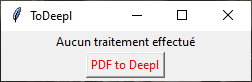
\includegraphics{data/ToDeepl.png}
	\caption{Fenêtre de ToDeepl}
	\label{fig_ToDeepl}
\end{figure}

\section{Utilisation}
\noindent
La fenêtre est constitué d'un seul bouton.\\

Lorsque du texte est copié depuis un document PDF (grâce au raccourcis ctrl+C), appuyer une fois sur le bouton permet de mettre en forme le texte directement dans le press papier de l'ordinateur.\\
Il est alors possible de le coller (ctrl+V) sur n'importe quel support.

	\subsection{Exemple}
Voici un text quelconque venant d'un PDF :
\begin{figure}[H]
	\centering 
	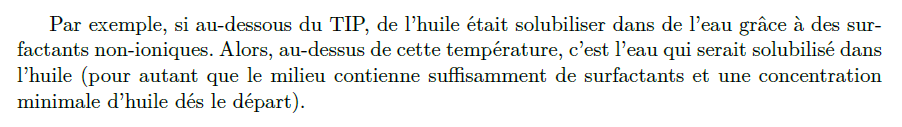
\includegraphics[width = \linewidth]{data/text_PDF.png}
	\caption{Texte quelconque venant d'un PDF}
	\label{fig_text_PDF}
\end{figure}

Résultat d'un simple copié coller dans un logiciel de traduction tel que Deepl :
\begin{figure}[H]
	\centering 
	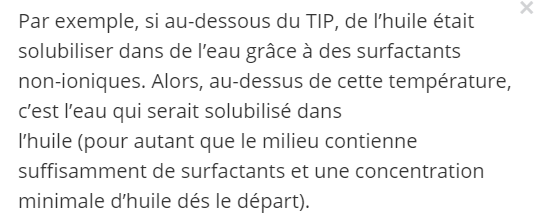
\includegraphics{data/text_sans_script.png}
	\caption{Copié coller sans utilisation du logiciel}
	\label{fig_text_sans_script}
\end{figure}
Le constat est frappant : les lignes sont coupées au milieu des phrases ce qui engendre une mauvaise traduction de la part d'un logiciel tel que Deepl par exemple.\\

Maintenant, le résultat en ayant utilisé le logiciel (Copié -> Utilisation de \enquote{ToDeepl} -> Coller) :
\begin{figure}[H]
	\centering 
	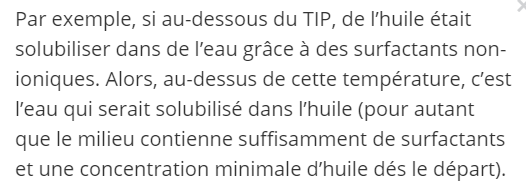
\includegraphics{data/text_script.png}
	\caption{Copié coller avec utilisation du logiciel}
	\label{fig_text_script}
\end{figure}
\noindent
Les phrases ne sont plus coupées !

\section{Remarque}
Le logiciel est prévu pour fonctionner correctement sous une installation Windows 10 possédant un interprètateur Python.\\

Si un autre système d'expoitation est installé sur votre ordinateur (Unix ou macOS par exemple) il se peut que le programme fonctionne correctement. Cependant, cela n'a pas été testé lors du développement.\\

Si vous ne possédez pas d'interprètateur  Python, il est aisé de l'installer en suivant ce lien : \url{https://www.python.org/downloads/}.

\end{document}